\documentclass{article}
\usepackage{graphicx}
\usepackage{wrapfig}
\usepackage{subcaption}
\usepackage[margin=1in]{geometry}
\usepackage{amsmath} % or simply amstext
\usepackage{siunitx}
\usepackage{booktabs}
\usepackage[export]{adjustbox}
\newcommand{\angstrom}{\textup{\AA}}
\newcommand{\colormap}{jet}  % colorbar to use
\usepackage{cleveref}
\usepackage{booktabs}
\usepackage{gensymb}
\usepackage{float}

\renewcommand{\thefigure}{S\arabic{figure}}
\renewcommand{\thesection}{S\arabic{section}}
\renewcommand{\thepage}{S\arabic{page}}
\renewcommand{\thetable}{S\arabic{table}}

\title{Supporting Information: Modeling Monomer Interactions with Molecular Dynamics}

\begin{document}

  \graphicspath{{./figures/}}
  \maketitle
  \bibliographystyle{ieeetr}

  We used an atomistic molecular model and molecular dynamics simulations 
  in order to quantify the number of acid-base reactions that would occur in
  a real system as a pure consequence of proximity. We ran all MD simulations
  and energy minimizations using GROMACS 2018.~\cite{bekker_gromacs:_1993,berendsen_gromacs:_1995,van_der_spoel_gromacs:_2005,hess_gromacs_2008}
  We built and equilibrated initial configurations and performed post-simulation trajectory 
  analysis using python scripts which are available online at \texttt{https://github.com/shirtsgroup/LLC\_Membranes}.
  Table~\ref{table:python_scripts} provides more detail about specific scripts
  used for each task.

  \begin{table}[htb!]
  \centering
  \newcolumntype{A}{m{2in}}
  \newcolumntype{C}{m{4in}}
  \begin{tabular}{|A|C|}
  \hline
  \multicolumn{1}{|c|}{\textbf{Script}}  & \multicolumn{1}{c|}{\textbf{Purpose}}                  \\ \hline
  
  \texttt{/setup/build.py}               & Build initial configuration                            \\ \hline
  \texttt{/setup/equil.py}               & Energy minimize and equilibrate initial configurations \\ \hline
  \texttt{/analysis/hbonds.py}           & Identify hydrogen bond interactions based on angle 
                                           and distance cut-off criteria.                         \\ \hline
  \texttt{/analysis/hbond\_reactions.py} & Track cumulative number of reacted acid-base pairs 
                                           using hydrogen bonds as a reaction surrogate           \\ \hline

  \end{tabular}

  \caption{The first column provides the names of the python scripts available in
  the \texttt{LLC\_Membranes} GitHub repository that were used for system setup and
  post-simulation trajectory analysis. Paths preceding script names are relative to the
  \texttt{LLC\_Membranes/LLC\_Membranes} directory. The second column provides a brief 
  description of the purpose of each script.}~\label{table:python_scripts}

  \end{table}
  
  We constructed four independent simulation unit cells on which to collect data.  
  The monoclinic unit cells consist of four pores, each made of 5 columns of 20
  monomers stacked on top of each other 3.7 \AA~apart in a parallel displaced 
  configuration (see Figure~\ref{fig:system_setup}). We randomly distributed the
  acidic and basic monomers among the columns. The parallel displaced $\pi-\pi$ 
  stacking configuration is more stable than the sandwiched configuration
  where monomers stack directly on top of each other.~\cite{sinnokrot_estimates_2002}
  In previous work with a similar monomer, we also found that systems built in the
  parallel displaced configuration as described above provide the closest match 
  to experimental structural data.~\cite{coscia_understanding_2019}

  \begin{figure}
  \centering
  \begin{subfigure}{0.34\textwidth}
  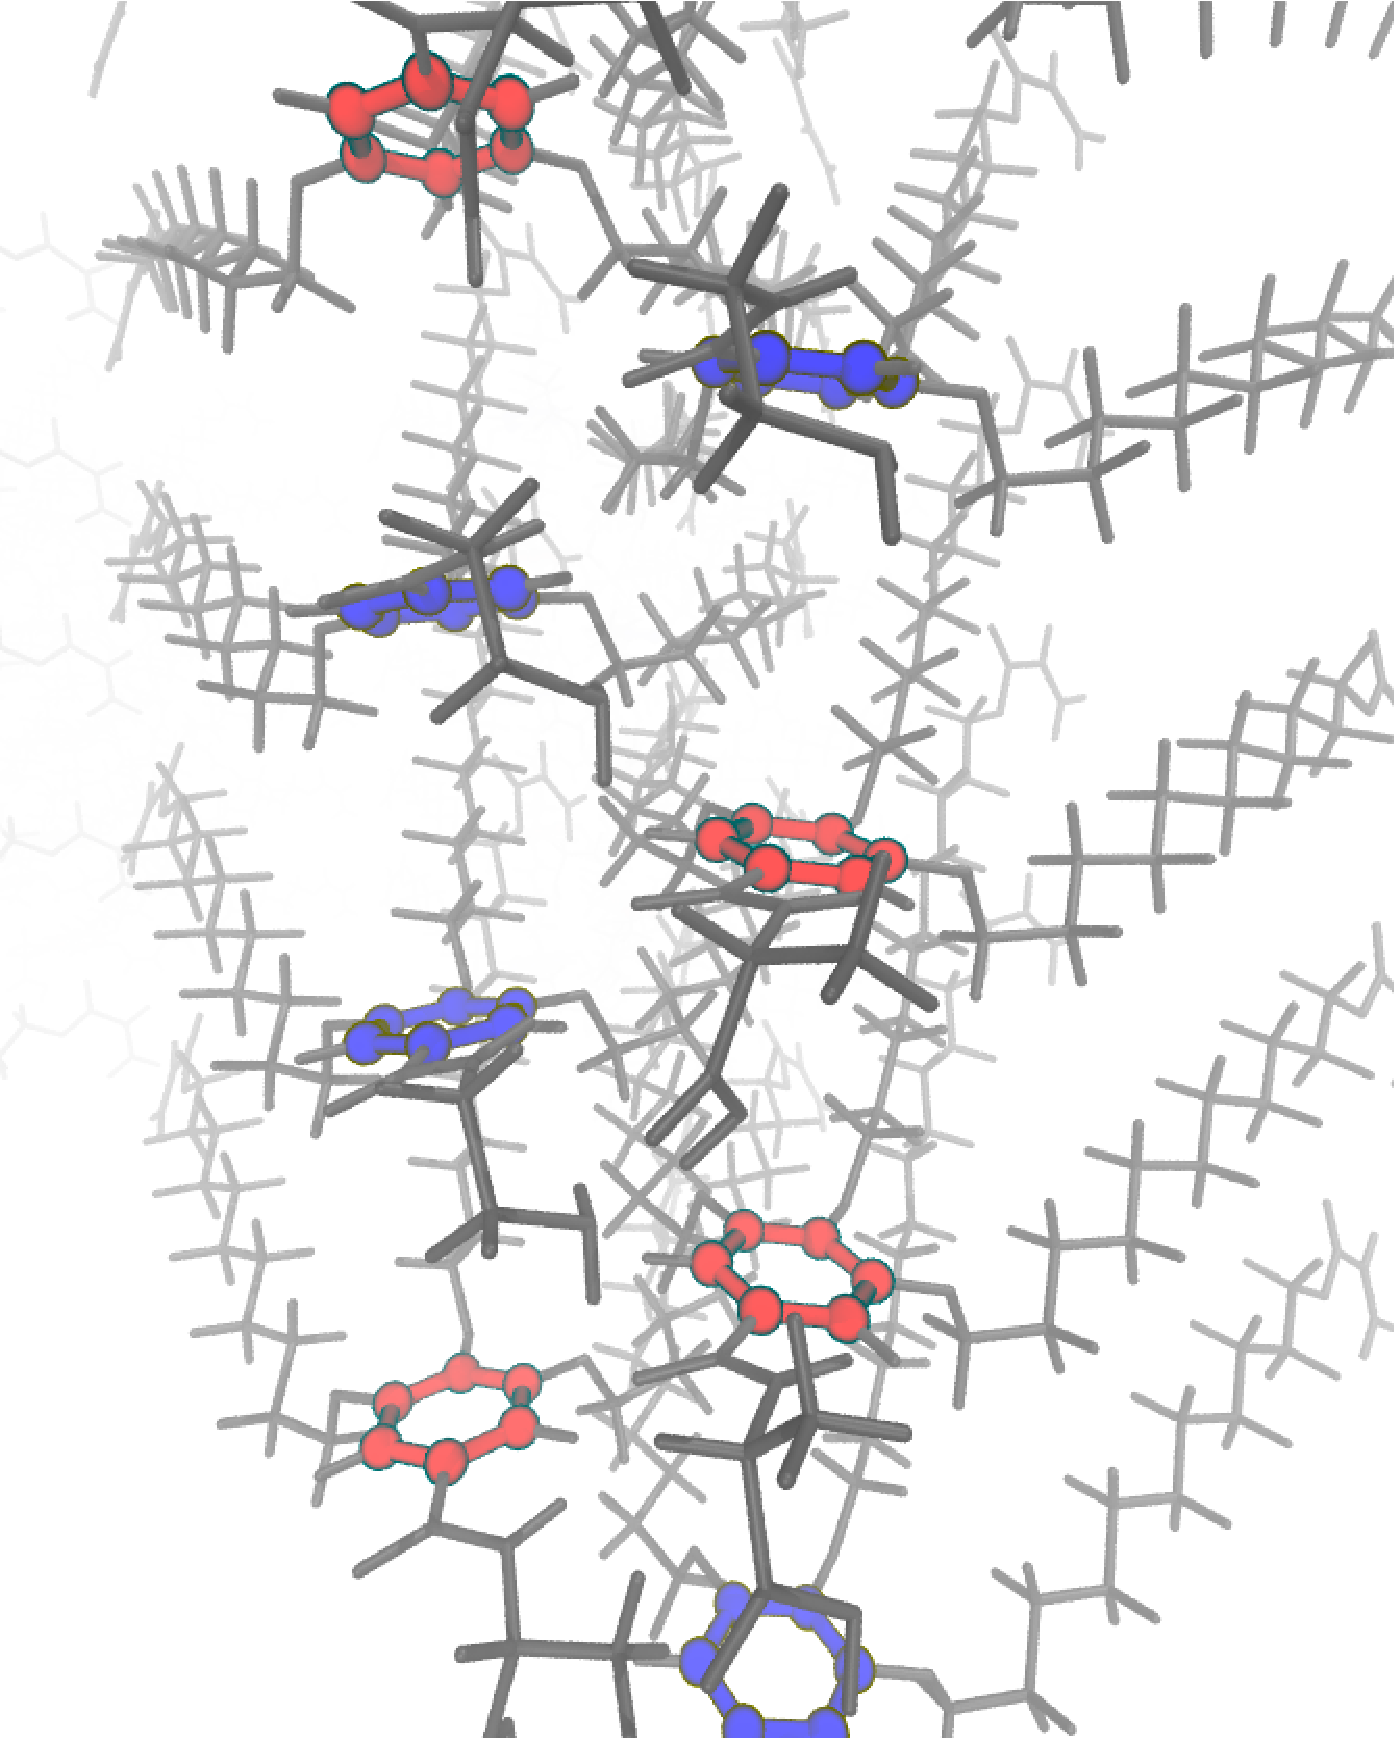
\includegraphics[width=\textwidth]{column.pdf}
  \caption{}\label{fig:column}
  \end{subfigure}
  \begin{subfigure}{0.56\textwidth}
  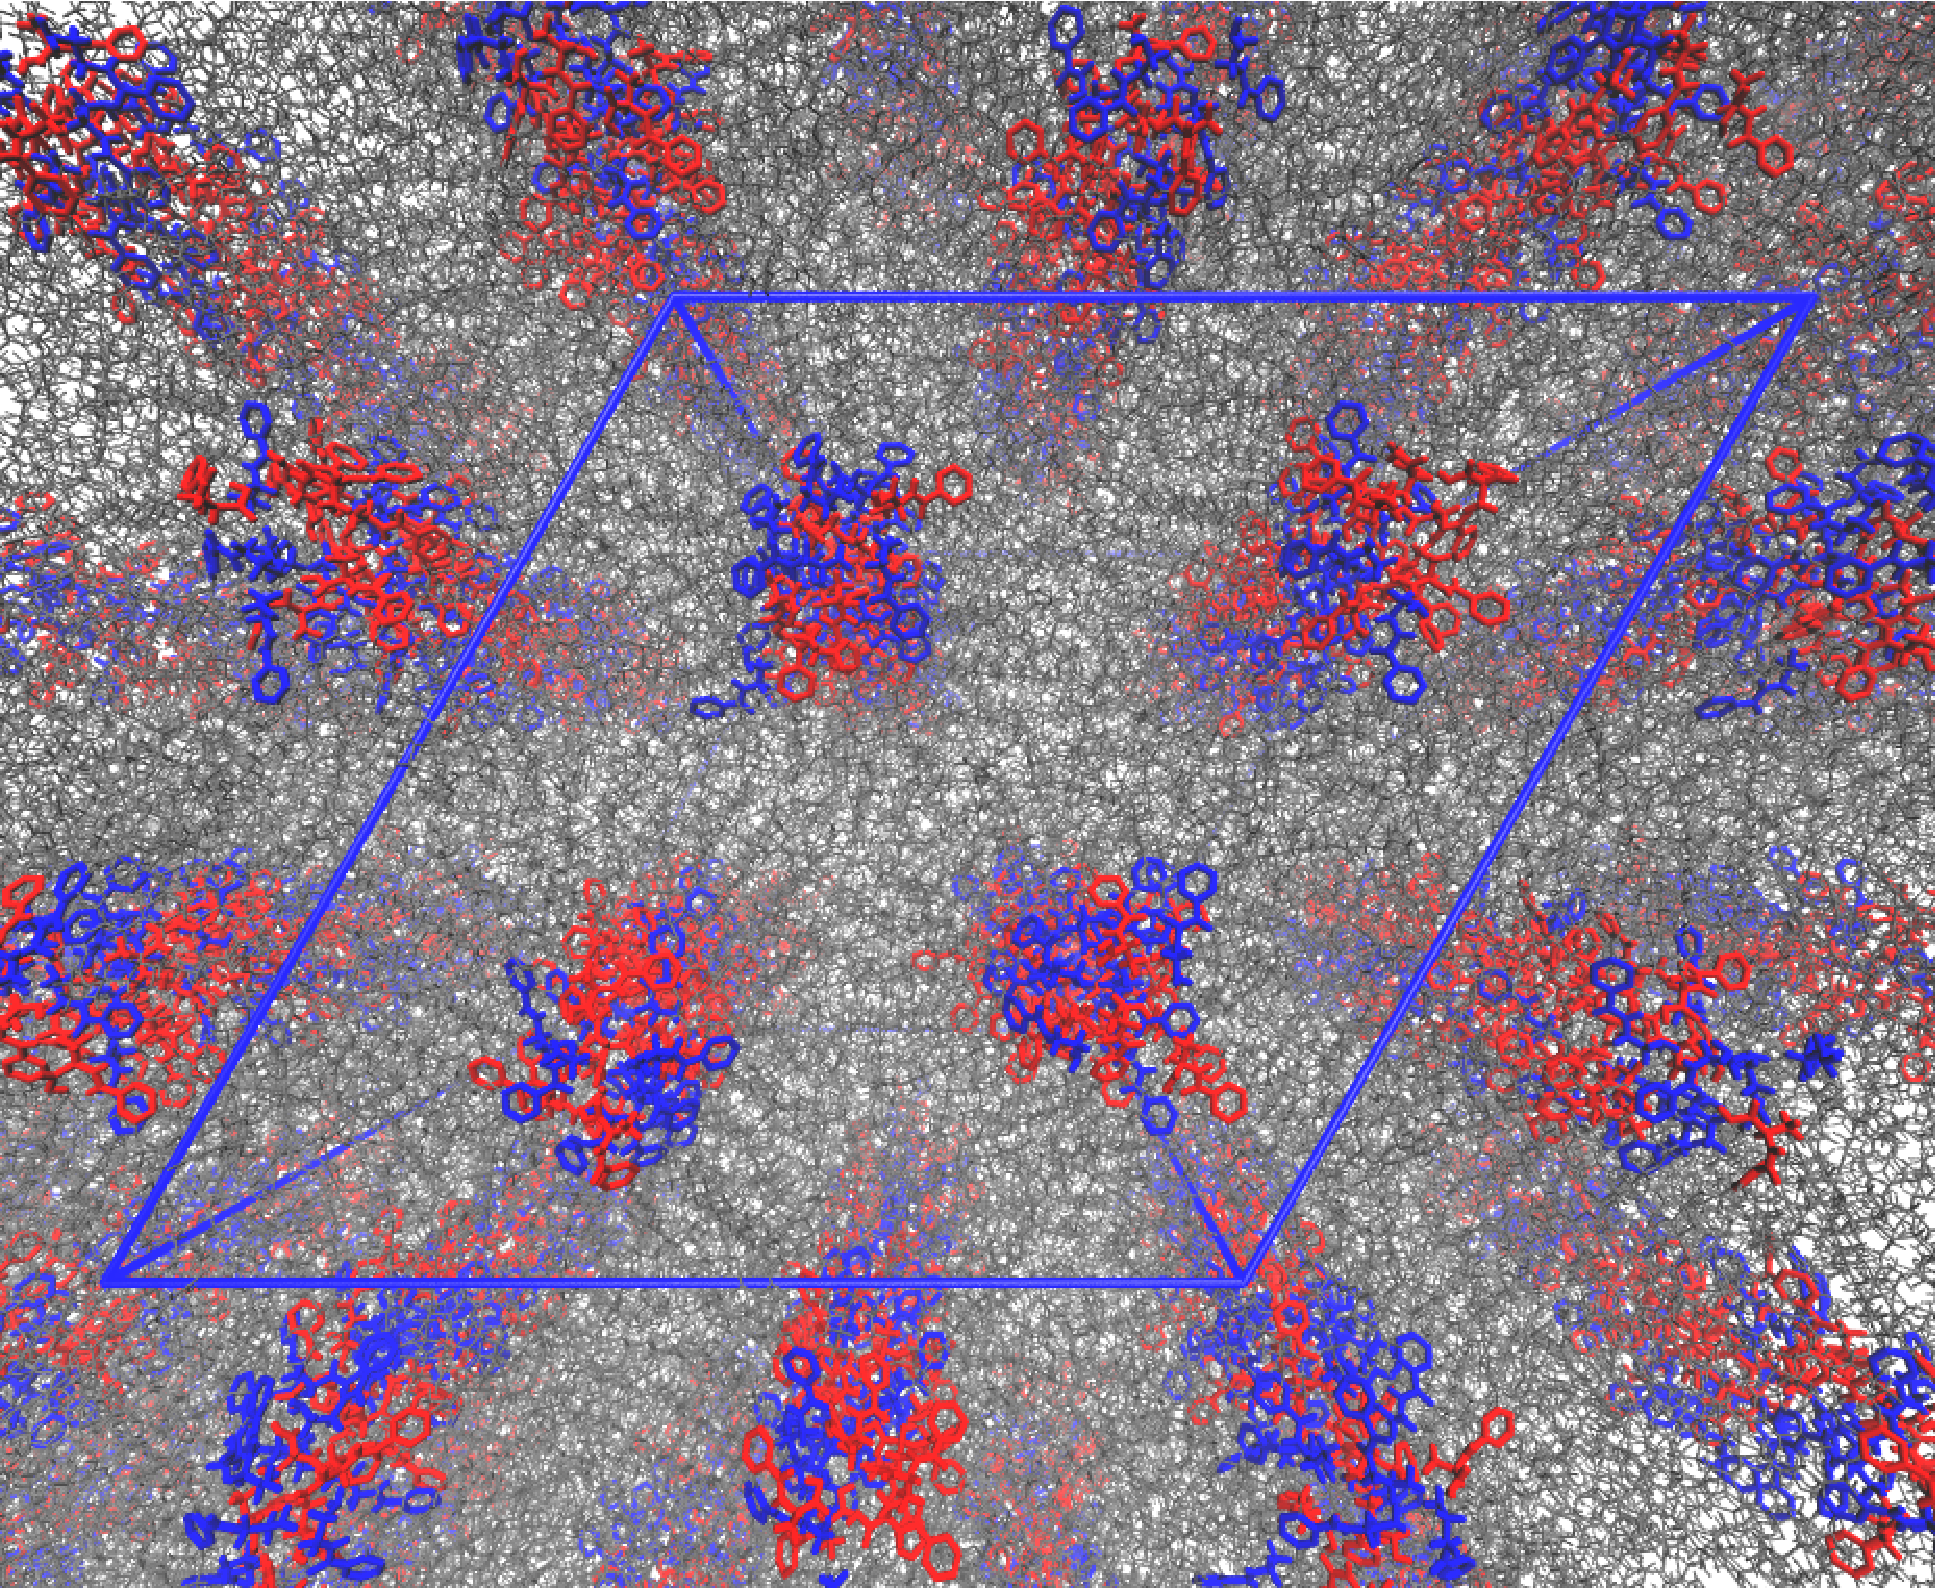
\includegraphics[width=\textwidth]{unitcell.pdf}
  \caption{}\label{fig:unitcell}
  \end{subfigure}
  \caption{(a) We randomly chose a total of 20 acidic (red) and basic (blue) 
  monomers and stacked the aromatic head groups in a parallel displaced 
  configuration on top of each other to form columns. (b) We created 4 pores, 
  each consisting of 5 columns, and placed them in a monoclinic unit cell (represented
  by the blue box) which is the smallest unit cell that preserves hexagonal 
  symmetry when the system is extended periodically. The pore centers are
  highlighted by the colored monomer head groups.}\label{fig:system_setup}
  \end{figure} 
  
  We equilibrated the unit cells using the same procedure as our previous
  work.~\cite{coscia_understanding_2019} All steps of the following
  procedure are implemented in \texttt{LLC\_Membranes/setup/equil.py} 
  (see Table~\ref{table:python_scripts}):
  % BJC: I can write this in paragraph form if that would be better.
  \begin{enumerate}
  	\item Build initial configuration
  	\item Energy minimize initial configuration with high (1e6 $\frac{kJ}{mol \cdot nm^2}$)
  	position restraints on head group heavy atoms. 
  	\item Run 50 ps NVT simulation with same position restraints.
  	\item Repeat steps 2 and 3, gradually reducing the force constant on head
  	group heavy atoms according to the sequence 3162, 56, 8, 3, 2, 1, 0 $\frac{kJ}{mol \cdot nm^2}$.
  	\item Run 5 ns unrestrained NPT simulation with semi-isotropic pressure 
  	coupling controlled by the Berendsen barostat and temperature controlled by the 
  	v-rescale thermostat.
  	\item Run long ($> 400~ns$) NPT simulations with semi-isotropic pressure
  	coupling controlled by the Parinello-Rahman barostat and temperature controlled by
  	the v-rescale thermostat.
  \end{enumerate}
  
  Because MD simulations typically do not involve reactions, we used hydrogen
  bonding as a surrogate for the acid-base reaction that would deactivate
  catalytic monomers. We considered a reaction to occur if a COOH group of monomer
  \textbf{1} donated its hydrogen to the NH\textsubscript{2} group of monomer
  \textbf{2}. A study of hydrogen bonding patterns among thousands of structures 
  in the Cambridge Structural Database suggests that this type of hydrogen
  bond does not exist~\cite{gilli_predicting_2009}. This is likely because proton
  transfer is immediate and nearly irreversible. % BJC: could put pKa calculation here 
  
  We predicted the percentage of unreacted monomers present in bulk film by
  counting the number of unique acid-base ``reactions'' as a function of time in 
  our MD simulations. In our search for hydrogen bonds, we considered each new 
  hydrogen bonded pair to be ``reacted'' and excluded both monomers from the rest
  of the search. 
  %We ran our simulations until the percentage of reacted monomers 
  plateaued for at least 100 ns.
  
  %As explained in the main text, clustering of acidic and basic monomers may prevent
  %an appreciable fraction of them from reacting with each other. 
  The exact percentage of unreacted monomers predicted from our simulations is a 
  function of the geometric criteria that we chose to use for identifying hydrogen bonds.
  There is no consensus in the simulation literature as to the proper way of identifying
  a hydrogen bond.~\cite{prada-gracia_quest_2013} In our previous work, we 
  defined a hydrogen bond to exist if the distance, $d$, between the donor (D) and acceptor (A)
  atoms was less than 3.5~\AA~and the D--H$\cdots$A angle, $\theta$, was less than 30\degree
  (see Figure~\ref{fig:hbond_geometry}).~\cite{coscia_chemically_2019} However, most
  of the hydrogen bonds were of the type O--H$\cdots$O whereas we are interested in
  O--H$\cdots$N. Studies of structurally similar hydrogen bonds show a range of 
  behavior with $d$ between 2.75 and 3.12 and $\theta$ up to 90\degree.~\cite{taylor_geometry_1984,haynes_hydrogen_2008}
  In the main text we chose to use $d$=3.0 and $\theta$=30\degree. We tested the 
  sensitivity of our conclusions to these criteria in Figure~\ref{fig:sensitivity}. 
  The plateau in the percentage reacted monomers is well below 100\% indicating that our
  conclusions hold with even the most lenient criteria.
  
  \begin{figure}
  \centering
  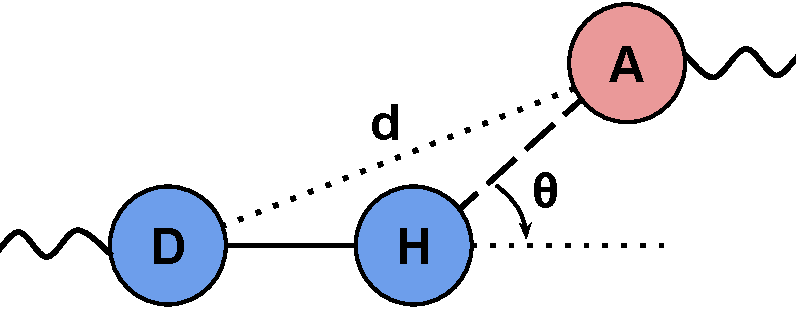
\includegraphics[width=0.5\textwidth]{hbond_geometry.pdf}
  \caption{We identify hydrogen bonds using geometric criteria based on
  the distance, $d$, between the donor (D) and acceptor (A) atoms as well
  as the angle, $\theta$, between the $\protect\overrightarrow{DH}$ and
  $\protect\overrightarrow{HA}$ vectors (where H is the hydrogen atom)}\label{fig:hbond_geometry}
  \end{figure}
  
  \begin{figure}
  \centering
  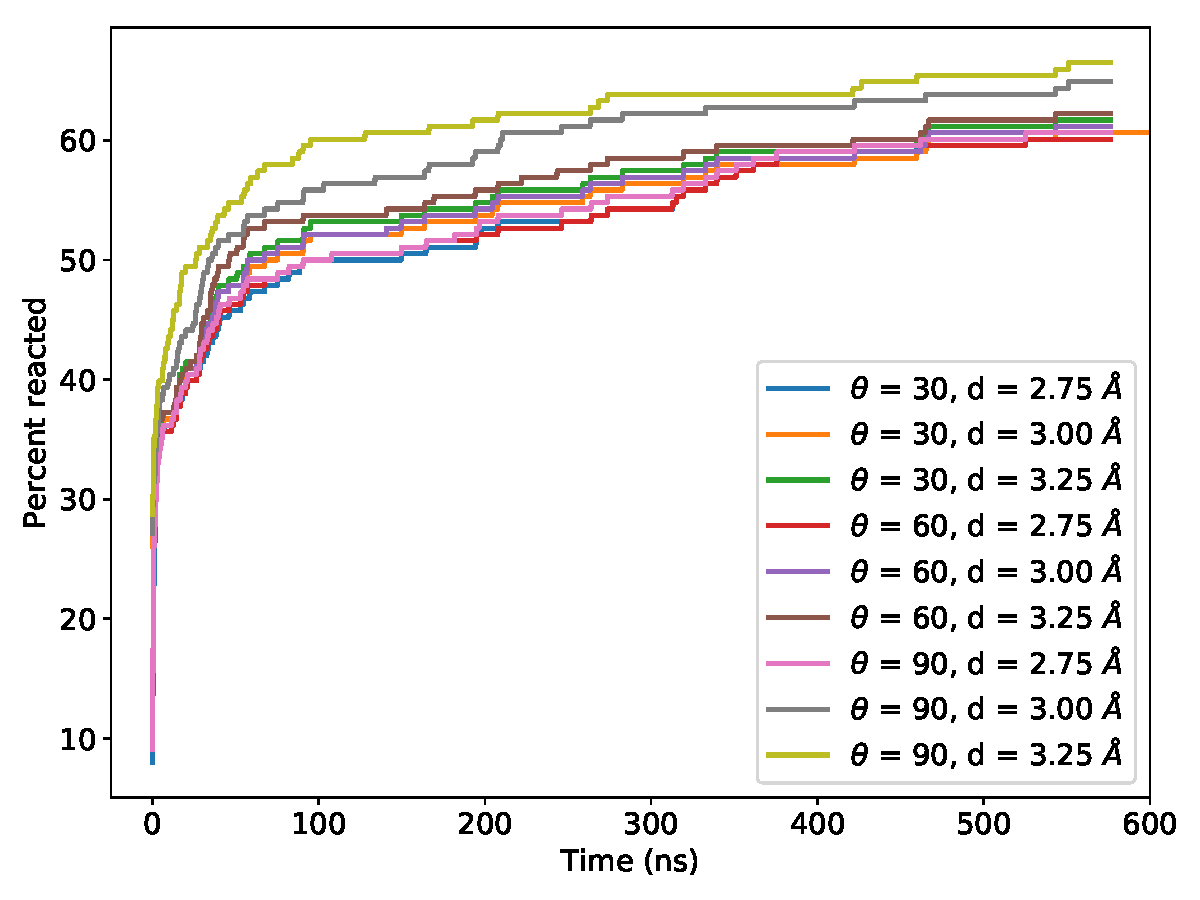
\includegraphics[width=0.65\textwidth]{sensitivity.pdf}
  \caption{We tested the sensitivity of our conclusions to hydrogen bond
  geometric identification criteria. As our conditions become more lenient
  (higher $d$ and $\theta$), the percentage of reacted monomers increases
  but still plateau's well below 100\%.}\label{fig:sensitivity}
  \end{figure}  
  
  We extrapolated the final number of reacted catalytic groups by fitting a
  plateauing function of the form:
  \begin{equation}
  f(x) = M(1 - x^{-a})
  \label{eqn:plateau}
  \end{equation}
  where $M$ and $a$ are the asymptotic maximum function value and the rate of
  decay respectively. We believe this type of fit is necessary because the 
  number of hydrogen bond "reactions" continues to grow slowly over time even
  after long plateaus (see Figure~\ref{fig:reacted_all}).
  
  There are multiple regimes of growth in the number of hydrogen bond surrogate
  reactions. Since we are interested in the asymptotic value, $M$, of the plateau,
  we fit Equation~\ref{eqn:plateau} to the average growth curve starting after
  40 ns where the percent reacted head groups versus the log of time becomes
  consistently linear (see Figure~\ref{fig:loglog}).
  
%  Because the system is very slowly approaching a plateau, we found that 
%  an $x^{-a}$ power law dependence in Equation~\ref{eqn:plateau} provided 
%  a better fit to the data than an exponential dependence ($e^{-ax}$) 
%  (see Figure~\ref{fig:fit_comparison}).
  
  \begin{figure}
  \centering
  \begin{subfigure}{0.45\textwidth}
  \includegraphics[width=\textwidth]{reacted_all.pdf}
  \caption{}\label{fig:reacted_all}
  \end{subfigure}
  \begin{subfigure}{0.45\textwidth}
  \includegraphics[width=\textwidth]{loglog.pdf}
  \caption{}\label{fig:loglog}
  \end{subfigure}
%  \begin{subfigure}{0.325\textwidth}
%  \includegraphics[width=\textwidth]{fit_comparison.pdf}
%  \caption{}\label{fig:fit_comparison}
%  \end{subfigure}
  \caption{(a) Although the growth rate of total surrogate reactions decreases 
  with time, it is likely that the curves will not fully plateau on a time scale
  that we can reasonably simulate. (b) The growth rate appears to enter at least
  three distinct regimes shown approximately by the different colored regions. We
  fit Equation~\ref{eqn:plateau} to the last (green) regime. 
  %(c) A power law 
  %growth rate ($x^{-a}$) gives a superior fit to our simulation data compared to
  %an exponential growth rate ($e^{-ax}$).
  }\label{fig:plateau}
  \end{figure}
  
  We used bootstrapping to determine the mean value of $M$ with its associated
  uncertainty. The procedure is as follows:
  \begin{enumerate}
  	\item Randomly choose, with replacement, 4 of the curves in Figure~\ref{fig:reacted_all}.
  	\item Fit Equation~\ref{eqn:plateau} to the mean of the 4 curves to get the value of $M$.
  	\item Repeat 200 times to generate a distribution of $M$ values. 
  	\item Report mean and standard error of $M$ distribution.
  \end{enumerate}
  Note that this procedure is best performed with many more than 4 curves, however
  it should still yield a more realistic uncertainty than the typically very small
  error returned by the single non-linear least squares fit to the average. 

  \pagebreak
  \bibliography{Catalysis}

\end{document}
